\section{Supporting Development Economics and Local Deployment}
\label{app:deployment}

\paragraph{Measured API requests.}
The exploratory report binds 452 requests (289 generator, 163 simulator)
to six rules-only runs and excludes 1,446 other or unbound ledger entries.
\autoref{fig:development-request-cost} retains run, provider and role counts.
All 452 have latency and settled all-in cost, including reported BYOK once.
Coverage includes every attempt status; unknown amounts remain missing.
Workloads differ. Requests within episodes are dependent; nearest-rank
p50/p95 summarize request round trips, rather than episode durations or
service guarantees.

\begin{figure}[htbp]
\centering
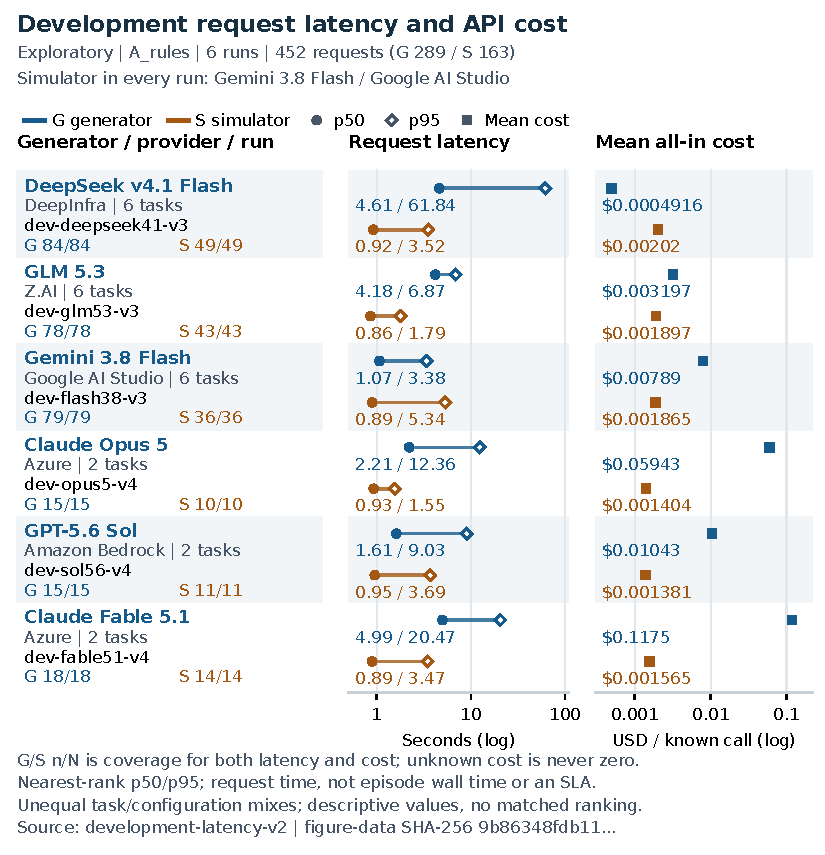
\includegraphics[width=\linewidth]{figures/development_request_latency_cost_compact.pdf}
\caption{Exploratory request latency and API cost by development run.
Blue denotes generator requests and orange denotes simulator requests
(Gemini~3.8 Flash through Google AI Studio in every run). Circles and diamonds
show p50/p95 latency; squares show mean all-in cost per known-cost call.
Both axes are logarithmic. G/S fractions give observed/attempted coverage
for both measures, separately for each role.}
\Description{Six shared development run rows retain all twelve generator and
simulator groups, their model and provider identities, latency percentiles,
mean known cost, role counts, and unequal two-task or six-task cohorts.}
\label{fig:development-request-cost}
\par\vspace{0.6em}
\begin{minipage}{\linewidth}
\small
\rule{\linewidth}{0.3pt}\par
\textbf{Illustrative budget for repeated cases.}
Suppose 100 cases each use five generator and five simulator calls per trial.
Three repeats then require 3,000 requests; eight require 8,000. Holding the
underlying unrounded role-specific mean charges fixed gives:
\par\vspace{0.3em}
\centering
\begin{tabular*}{0.96\linewidth}{@{\extracolsep{\fill}}lrr@{}}
\toprule
Generator & 100 cases $\times$ 3 repeats & 100 cases $\times$ 8 repeats \\
\midrule
DeepSeek v4.1 Flash & \$3.77 & \$10.05 \\
GLM 5.3 & \$7.64 & \$20.38 \\
Gemini 3.8 Flash & \$14.63 & \$39.02 \\
Claude Opus 5 & \$91.25 & \$243.34 \\
GPT-5.6 Sol & \$17.72 & \$47.26 \\
Claude Fable 5.1 & \$178.64 & \$476.37 \\
\bottomrule
\end{tabular*}
\par\vspace{0.3em}
\raggedright
DeepSeek and GLM are hosted open-weight routes here. Each row uses its own
observed Gemini simulator mean. The assumed call counts and unchanged
prompt/output, caching and provider mix define this arithmetic scenario;
additional gate calls are excluded. Unequal development workloads limit
quality-adjusted comparisons.
\end{minipage}
\end{figure}

\begin{figure}[htbp]
\centering
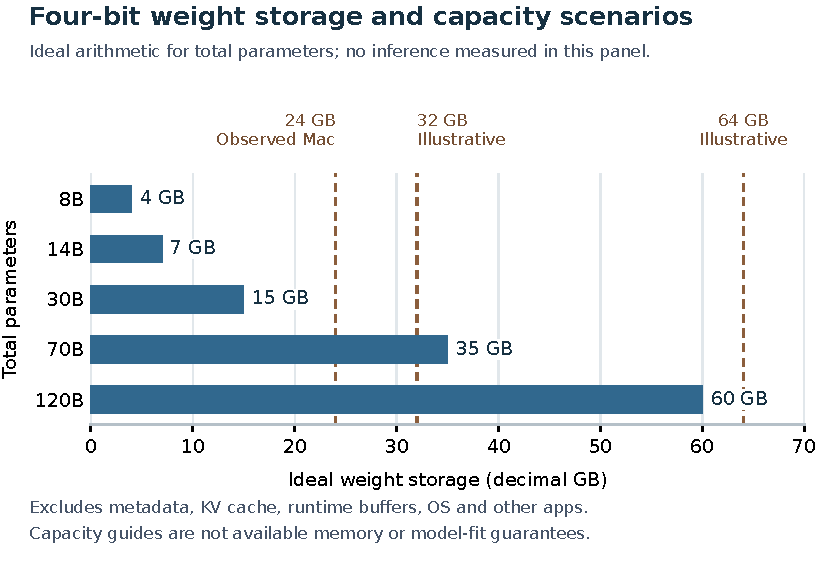
\includegraphics[width=\linewidth]{figures/local_weight_storage_paper.pdf}
\caption{Ideal four-bit weight storage, computed from total parameters,
including stored mixture-of-experts parameters. The 24~GB guide marks the
observed Mac; 32/64~GB are illustrative device-capacity scenarios. A full memory
budget also includes quantization metadata, higher-precision tensors, KV cache,
runtime buffers, operating-system and other application memory. These scenarios
support memory sizing for the local qualification; model fit, serving throughput
and workload quality require runtime qualification.}
\Description{Ideal weight storage for 8, 14, 30, 70 and 120 billion total
parameters, with 24, 32 and 64 GB capacity guides.}
\label{fig:local-weight-storage}
\par\vspace{0.6em}
\begin{minipage}{\linewidth}
\small
\rule{\linewidth}{0.3pt}\par
\textbf{Measured local technical qualification.}
On the owned M4 Pro MacBook Pro with 24~GB memory, six preselected
Granite~4.2 3B calls through Ollama~0.34.2 produced technically valid structured
outputs. Observed request latency ranged from 3.197 to 6.201 seconds
(mean 4.344); resident-model telemetry was approximately 3.050~GB.
Four calls reported caching. Context retention and inference freshness
remain unqualified, and correctness remains unscored. This six-call local
qualification is reported separately from the API cohorts.
Local API charges were zero; energy and hardware amortization were unmeasured.
\par\medskip
\textbf{Ownership-cost scenarios.}
For an already-owned Mac, the purchase is sunk for a current incremental
inference decision. A new deployment comparison must separately account for
purchase or amortization, utilization, energy, maintenance and replacement.
The comparison should measure serving throughput, workload quality and
evidence preservation alongside cost, with action controls validated for the
target workflow.
\end{minipage}
\end{figure}
